\documentclass[chi_draft]{sigchi}

% Use this section to set the ACM copyright statement (e.g. for
% preprints).  Consult the conference website for the camera-ready
% copyright statement.

% Copyright
\CopyrightYear{2018}
%\setcopyright{acmcopyright}
\setcopyright{acmlicensed}
%\setcopyright{rightsretained}
%\setcopyright{usgov}
%\setcopyright{usgovmixed}
%\setcopyright{cagov}
%\setcopyright{cagovmixed}
% DOI
\doi{http://dx.doi.org/10.475/123_4}
% ISBN
\isbn{123-4567-24-567/08/06}
%Conference
\conferenceinfo{ASSETS'18,}{October 22--24, 2018, Galway, Ireland}
%Price
\acmPrice{\$15.00}

% Use this command to override the default ACM copyright statement
% (e.g. for preprints).  Consult the conference website for the
% camera-ready copyright statement.

%% HOW TO OVERRIDE THE DEFAULT COPYRIGHT STRIP --
%% Please note you need to make sure the copy for your specific
%% license is used here!
% \toappear{
% Permission to make digital or hard copies of all or part of this work
% for personal or classroom use is granted without fee provided that
% copies are not made or distributed for profit or commercial advantage
% and that copies bear this notice and the full citation on the first
% page. Copyrights for components of this work owned by others than ACM
% must be honored. Abstracting with credit is permitted. To copy
% otherwise, or republish, to post on servers or to redistribute to
% lists, requires prior specific permission and/or a fee. Request
% permissions from \href{mailto:Permissions@acm.org}{Permissions@acm.org}. \\
% \emph{CHI '16},  May 07--12, 2016, San Jose, CA, USA \\
% ACM xxx-x-xxxx-xxxx-x/xx/xx\ldots \$15.00 \\
% DOI: \url{http://dx.doi.org/xx.xxxx/xxxxxxx.xxxxxxx}
% }

% Arabic page numbers for submission.  Remove this line to eliminate
% page numbers for the camera ready copy
% \pagenumbering{arabic}

% Load basic packages
\usepackage{balance}       % to better equalize the last page
\usepackage{graphics}      % for EPS, load graphicx instead 
\usepackage[T1]{fontenc}   % for umlauts and other diaeresis
\usepackage{txfonts}
\usepackage{mathptmx}
\usepackage[pdflang={en-US},pdftex]{hyperref}
\usepackage{color}
\usepackage{xspace}
\usepackage{booktabs}
\usepackage{textcomp}

% Some optional stuff you might like/need.
\usepackage{microtype}        % Improved Tracking and Kerning
% \usepackage[all]{hypcap}    % Fixes bug in hyperref caption linking
\usepackage{ccicons}          % Cite your images correctly!
% \usepackage[utf8]{inputenc} % for a UTF8 editor only

% If you want to use todo notes, marginpars etc. during creation of
% your draft document, you have to enable the "chi_draft" option for
% the document class. To do this, change the very first line to:
% "\documentclass[chi_draft]{sigchi}". You can then place todo notes
% by using the "\todo{...}"  command. Make sure to disable the draft
% option again before submitting your final document.
\usepackage{todonotes}

% Paper metadata (use plain text, for PDF inclusion and later
% re-using, if desired).  Use \emtpyauthor when submitting for review
% so you remain anonymous.
\def\plaintitle{Leveraging Augmented Reality Technology for Orientation and Mobility Apps for People with Visual Disabilities}
\def\plainauthor{First Author, Second Author, Third Author,
  Fourth Author, Fifth Author, Sixth Author}
\def\emptyauthor{}
\def\plainkeywords{visual disability; orientation and mobility; augmented reality; assistive technology; smartphone apps}
\def\plaingeneralterms{Documentation, Standardization}

% llt: Define a global style for URLs, rather that the default one
\makeatletter
\def\url@leostyle{%
  \@ifundefined{selectfont}{
    \def\UrlFont{\sf}
  }{
    \def\UrlFont{\small\bf\ttfamily}
  }}
\makeatother
\urlstyle{leo}

% To make various LaTeX processors do the right thing with page size.
\def\pprw{8.5in}
\def\pprh{11in}
\special{papersize=\pprw,\pprh}
\setlength{\paperwidth}{\pprw}
\setlength{\paperheight}{\pprh}
\setlength{\pdfpagewidth}{\pprw}
\setlength{\pdfpageheight}{\pprh}

% Make sure hyperref comes last of your loaded packages, to give it a
% fighting chance of not being over-written, since its job is to
% redefine many LaTeX commands.
\definecolor{linkColor}{RGB}{6,125,233}
\hypersetup{%
  pdftitle={\plaintitle},
% Use \plainauthor for final version.
%  pdfauthor={\plainauthor},
  pdfauthor={\emptyauthor},
  pdfkeywords={\plainkeywords},
  pdfdisplaydoctitle=true, % For Accessibility
  bookmarksnumbered,
  pdfstartview={FitH},
  colorlinks,
  citecolor=black,
  filecolor=black,
  linkcolor=black,
  urlcolor=linkColor,
  breaklinks=true,
  hypertexnames=false
}


\newcommand{\BVI}{B/VI\xspace}
\newcommand{\OM}{O\&M\xspace}

% create a shortcut to typeset table headings
% \newcommand\tabhead[1]{\small\textbf{#1}}

% End of preamble. Here it comes the document.
\begin{document}

\title{\plaintitle}

\numberofauthors{3}
\author{%
  \alignauthor{Leave Authors Anonymous\\
    \affaddr{for Submission}\\
    \affaddr{City, Country}\\
    \email{e-mail address}}\\
  \alignauthor{Leave Authors Anonymous\\
    \affaddr{for Submission}\\
    \affaddr{City, Country}\\
    \email{e-mail address}}\\
  \alignauthor{Leave Authors Anonymous\\
    \affaddr{for Submission}\\
    \affaddr{City, Country}\\
    \email{e-mail address}}\\
}

\maketitle

\begin{abstract}
With the introduction of augmented reality technology to the iOS and Android platforms, mainstream smartphones now have the ability to track the motion of a user's phone in 3D space with high accuracy.  Here, we present our work leveraging these new capabilities to create two smartphone apps for people with visual disabilities: (1) an app that provides automatic navigation guidance when backtracking along a route and (2) an app that leverages crowdsourcing to misplaced objects.  Along with a discussion of the design of the apps themselves, we present a preliminary usability study that supports their utility.  We conclude with a discussion of the promises and limitations of augmented reality smartphone technology to create assistive apps for people with visual disabilities.
\end{abstract}

\category{K.4.2.}{Assistive technology for persons with disabilities}{Orientation and mobility tools for people who are blind or visually impaired}

\keywords{\plainkeywords}

\section{Introduction}

For people who are blind or visually-impaired (\BVI), improvements in orientation and mobility (\OM) have been shown to increase economic opportunity as well as psychological well-being.  While only 30\% of working-age Americans who are \BVI are employed \cite{employmentstatistics2017, kirchner1999looking} (compared with 65\% of the general population), individuals with better \OM skills have a higher likelihood of being employed \cite{crudden1998comprehensive, crudden1999barriers, leonard1999factors, o1999employment}.   Similarly, while the link between visual-impairment and depression has been well-documented \cite{rubin1994visual, rovner1996depression, hayman2007depression, heyl2001psychosocial}, several studies have suggested that it is disability rather than blindness itself that is at the root of this linkage \cite{rovner1996depression, williams1998psychosocial}.  For example, it was found that one's ability to perform daily-life tasks, such as shopping for basic necessities, was \emph{more} predictive of overall life satisfaction than was degree of vision loss \cite{williams1998psychosocial}.

Due to its high degree of importance, there is a long history of engineers creating assistive technology to empower people are \BVI to perform \OM tasks more easily (see the \emph{Background and Related Work} section for a discussion of this).  Here, we explore new technological developments and trends, which are enabling the development of widely accessible assistive technology for \OM.  The first enabling trend is the high rate of ownership of smartphones by people who are \BVI \cite{morris2014blind}.  The availability of these devices has already had revolutionary impacts on accessibility (e.g., through GPS-based directions, OCR software).  The second driver of this trend is the introduction of high accuracy 3D-tracking capabilities into mainstream smartphones.  While the primary purpose of these modules, e.g., Apple's ARKit \cite{arkit}, Google's ARCore \cite{arcore}, is to enable augmented reality applications, whereby virtual and real world content are mingled, e.g., by overlaying images on a smartphone video feed, these modules can be repurposed to create very powerful assistive technology for \OM.

In this document we present our work on leveraging the augmented reality modules in modern smartphones to create assistive technologies to help users who are blind with everyday \OM tasks.  In service of our goal of designing impactful technologies, we employed user-centered design principles throughout the research and development lifecycle, including working longitudinally with a co-designers who are blind.  Further, two of the study authors, who have severe visual impairments, contributed to all aspects of the project and additionally provided much needed design guidance to the project based on their personal experiences.

Our first app is called Clew, and it enables users to backtrack along previously traveled routes.  This capability is designed to help with various pain points experienced by non-visual travelers, including finding one's way independently after being brought to a location by a sighted guide.  The second app is called View Share, which utilizes crowdsourcing to enable a user to find objects and receive automated guidance to objects in cluttered environments.  In the remainder of the paper we provide some relevant background and related work on \OM assistive technology, discuss some of the algorithms that underlie the AR technology of modern smartphones, discuss our two developed apps in detail, provide preliminary usability, and finally conclude with a discussion of future challenges and promising directions of smartphone-based AR technology for people who are \BVI.   \todo{Need to sell harder in the intro once the story of the paper becomes more complete.  For example, listing out the three most important contributions of this paper.}

\section{Background and related work}
Engineers have long sought to use technology to improve the \OM capabilities of people who are \BVI.  Most of the early work in this area has focused on the usage of technology to help with things such as obstacle detection and avoidance.  For example, researchers have created obstacle-detecting versions of the long cane by instrumenting it with sensors such as lasers \cite{benjamin1973new} and sonar \cite{borenstein1997guidecane}.  These sorts of devices based around obstacle detection have not achieved high adoption by the \BVI community for a number of reasons, including their cost, lack of reliability, and limited new functionality over the white cane (see \cite{wiener2010foundations} for a discussion of this issue).

Recently, spurred by the high ownership rates of smartphones among people who are \BVI, the focus of this work has shifted from obstacle avoidance problems such as navigation and spatial awareness.  For instance, GPS-based navigation apps, such as BlindSquare \cite{blindsquare} and Google Maps, allow users who are \BVI to navigate to destinations of interest and learn about nearby landmarks and businesses.  The combination of location awareness, as provided by GPS, along with extensive databases of businesses, streets, and points of interest have allowed these apps to provide high-quality assistance to people who are \BVI.

GPS-based apps for \OM have a number of limitations, including limited accuracy (in good conditions GPS on smartphones is accurate to about $10m$, and can be much less accurate in urban environments) and lack of function inside.  To circumvent these challenges, researchers are pursuing largely two major approaches.  The first approach is to utilize crowdsroucing, whereby people who are \BVI connect with a sighted person for on-demand assistance.  Crowdsourcing has a successful track record in the area of assistive tech (e.g., the highly successful VizWiz project \cite{bigham2010vizwiz}) and this same model has been used by the BeMyEyes app \cite{bemyeyesaccessworld} and the Aira system \cite{aira}, which each connect a user who is \BVI with a sighted volunteer through a video chat interface.  The second approach is to utilize  along with inertial sensing (e.g., accelerometers and gyroscopes) to enable accurate positioning (both indoors and outdoors).  The second class of apps combine rudimentary (and somewhat inaccurate) motion estimation via inertial sensors (gyroscopes and accelerometers) along with special environmental infrastructure (e.g., Bluetooth-enabled location beacons) that provide sporadic location cues to enable relatively accurate indoor positioning.  For instance, \cite{ganz2015percept, ganz2011percept, ganz2014percept} developed a system for navigating indoor environments using smartphone-detectable RFID tags.  Dias and her collaborators utilized WiFi fingerprinting (calibrated using a highly-precise indoor mapping robot) and dead-reckoning (using the accelerometers and gyroscopes on a standard smartphone) for indoor navigation \cite{Dias__2014_7778}.  A similar system uses low-energy Bluetooth beacons instead of WiFi access points as landmarks \cite{ishihara2017beacon, ahmetovic2016navcog, ahmetovic2017achieving}.  A third approach is to utilize a calibrated database containing images at known locations, which are then matched to camera images at run time \cite{bai2014wearable}.\todo{figure out a place to integrate some of Aaron Steinfeld's work}

\section{Augmented Reality}

\begin{figure}
\begin{center}
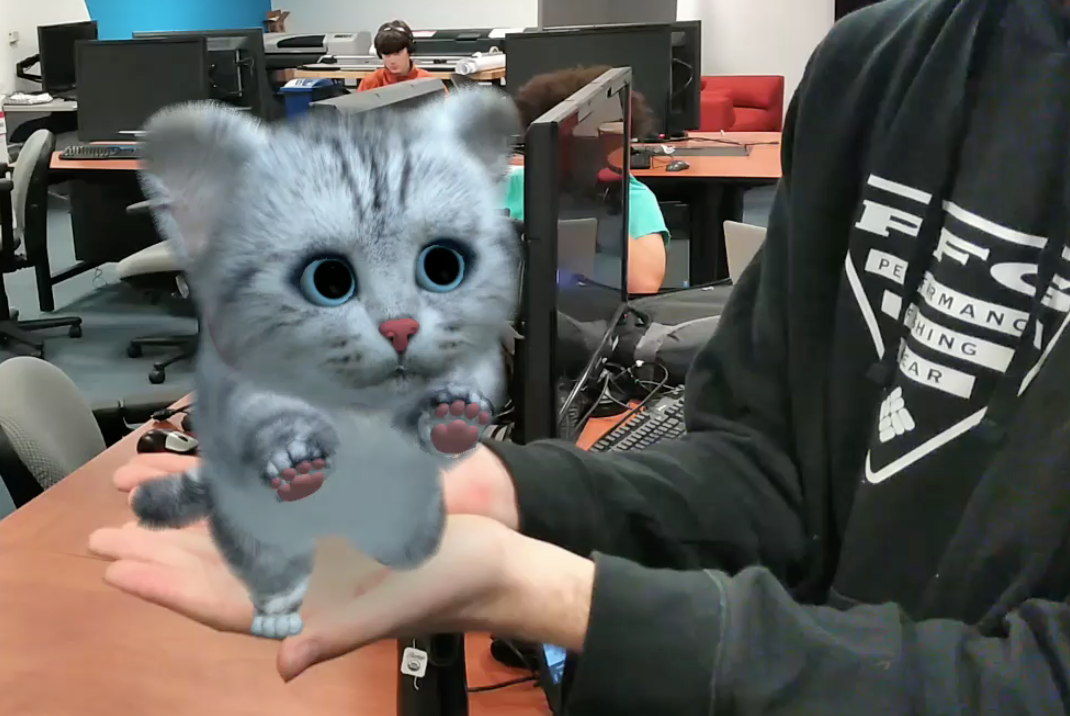
\includegraphics[width=.9\linewidth]{Figures/arexample.png}
\end{center}
\caption{A virtual cat overlaid on a smartphone camera feed.  The phone is able to accurately sense its movement in order to render the cat at the appropriate viewing angle and depth.\label{fig:arexample}}
\end{figure}

Recently, both Apple and Google have begun to rollout significant new capabilities that enable users to enjoy highly sophisticated augmented reality (AR) experiences on their smartphones.  The key characteristic of AR-enabled apps is that virtual content is seamlessly combined with real world content.  The most common instantiation of this idea is to overlay virtual objects or characters on top of the video feed form a smartphone.  For instance, Figure~\ref{fig:arexample} shows a virtual cat that is projected into a real world scene.  As the user moves around in the space, the phone will detect the user's motion with high accuracy and automatically render the cat from an appropriate angle and distance, providing the illusion that the cat exists in the physical world.

These new AR systems are made possible by spatial processing algorithms that are vastly more accurate than the simple inertial-based systems utilized in pervious assistive \OM apps.  The high accuracy of these systems has been driven by two key trends: the development of sophisticated algorithms for visual-inertial odometry (VIO) \cite{li2013high,leutenegger2015keyframe,bloesch2015robust,forster2014svo} (which combine optical tracking using a smartphone's camera with inertial sensing for motion estimation) and the development of special purpose hardware that allows these highly computationally intensive algorithms to run on a user's smartphone with minimal heat generation and power consumption.  The high-degree of motion estimation accuracy enabled by these systems, unlocks many new possible \OM apps for people who are \BVI, which we will described later.

\subsection{Algorithms for Visual Inertial Odometry}
In order to understand the potential of VIO for creating assistive \OM applications, it helps to understand a bit about how these algorithms function.  A full explanation of VIO is beyond the scope of this document.  For a more comprehensive treatment consult \cite{gui2015review}.  Approaches for VIO have been developed for both the stereo setting and the monocular (or single camera) setting.  The monocular setting is directly applicable to most modern smartphones, which either only have one rear-facing camera or have a second camera that is unsuitable for use in a stereo pair.  For the remainder of this section, we'll focus on the monocular case only.

VIO algorithms utilize sensor fusion to blend motion estimates generated by a camera and an IMU.  An estimate of the motion of a camera can be made by tracking salient visual features (for instance, corners or other highly textured portions of the image) over the course of multiple frames.  Utilizing the mathematics of perspective geometry, one can estimate the rotation and translation of the camera based on the global pattern of movement of these visual features \cite{Hartley2004}.  Of particular interest to the creation of assistive apps-based on this technology, the accuracy of these motion estimates is highly dependent on being able to track a large number of these visual features that ideally correspond to points at a range of distances from the camera and are distributed uniformly over the image.  This dependency means that VIO is susceptible to inaccurate motion tracking when few visual features are able to be tracked frame-to-frame or when the visual features that are tracked represent are impoverished (e.g., all at the same depth or in the same region of the image).  While some environments are simply more difficult for visual tracking, in some cases users may hold their phones in a suboptimal position (e.g., with the camera facing the ground).  Assuming a suitable set of visual features is tracked, the motion estimates of the translation of the camera are only determined up to an arbitrary scale factor.  This problem is known as scale indeterminacy.  This indeterminacy arises due to the fact that the depths (perpendicular distance from the image plane) of the visual features are unknown \cite{Hartley2004}.  For example, for any particular estimate of the translation of the camera, it is equally valid that the camera moved twice as far and the depths of the visual features were all twice as great.

The shortcomings of motion estimates from optical tracking, scale-indeterminacy and inaccurate performance in feature-poor environments, can be overcome (to some degree) by the fusion of inertial sensing data (gyroscopes and accelerometers).  Gyroscopes, which provide accurate estimates of angular velocity over short timescales, can be used to refine the estimate of rotation generated by visual tracking and accelerometer data can be integrated to obtain an estimate of linear velocity to overcome the scale-indeterminacy problem.  Since inertial sensors don't function optimally when subjected to extremely fast rotations or high accelerations, users need to hold their phones relatively stable to get the full benefits of VIO.

\subsection{VIO in Mass-Market Smartphones}
Both Apple and Google have released AR modules based on VIO.  Unfortunately, the precise details of the algorithms employed by each platform are not publicly available, however, their are important high-level differences in these implementations for application developers to keep in mind.

\subsubsection{Google Tango}
The Google Tango platform was first made publicly available by Google's ATAP (Advanced Technology and Projects) division in late 2014.  Google's platform utilized a special wide angle (fisheye) camera equipped with a global (more precise) shutter that enabled maximally accurate visual feature tracking.  Further, the platform included a PrimeSense depth-sensing camera, although the depth sensor was not utilized to estimate the motion of the phone.  Two commercial products have been released based on the Google Tango technology: the Lenovo Phab2 Pro and the Asus Zenfone AR.  While the tracking capabilities of Tango devices is superior to other platforms (discussed next), the reliance of the platform on special-purpose hardware severely limited the adoption of the technology, leading Google to suspend the project in March of 2018 \cite{tangoretired}.


\subsubsection{ARKit and ARCore}

Apple's ARKit \cite{arkit} and Google's ARCore \cite{arcore}, both released in 2017, provide AR-capabilities that do not require special purpose cameras.  Since these platforms utilize conventional cameras, the richness of visual features available for tracking is not as high as those that can be harvested from fisheye lens on Tango platforms.  Based on our anecdotal observation, this results less accurate tracking performance than the Tango.  Further, since neither of these platforms have built-in depth sensing cameras, the availability of 3D information about the landmarks in the environment is limited to objects with special structure (e.g., horizontal and vertical planes).  Of primary importance is that these frameworks are capable of running on a much wider share of phones than Google Tango.  Further, given the much higher preference for iOS devices by people who are \BVI \cite{morris2014blind}, ARKit is the primary platform of interest for researchers seeking to develop assistive apps based on smartphone-based AR technology.

\section{User-Centered Design Process}
\todo{might want to put this later.  The paper could run the risk of dragging at this point}
My lab has been working to develop \OM assistive technology for the last several years.  We take a user-centered approach in which we deeply engage with people who are \BVI to understand their needs, wants, and values as well as any pain points and areas of opportunity that exist within their daily lives.  As such, we've used a mixture of quantitative and qualitative methods to arrive at problem spaces along with ideas for assistive technologies to help with \OM.

\subsection{Identified Areas of Opportunity}
Based on both our background research along with our interviews and observation of individuals who are \BVI, we identified several areas of opportunity for the development of assistive apps.  The themes of high precision and indoor navigation came up again and again in our interactions with users.  Further, the notion of being able to browse (for instance in a grocery store or other public space) was also something that was repeatedly identified by our participants.  Finally, users expressed a desire to more quickly build facility in navigating, independently, through unfamiliar environments.

\subsection{Usability Factors of VIO Technology}
Based on the identified areas of opportunity, along with the emerging implementation of VIO on modern smartphones, it was natural to investigate the suitability of these approaches.  Since VIO is a sensor-fusion algorithm that relies, in part, on visual tracking, any assistive app based on VIO must maintain the condition that the user's smartphone's camera is unoccluded.  In the designs explored in this paper, we assume that the user would hold the phone in one hand while holding their long cane in the other.  In some cases the user may require handsfree operation of their smartphone. The development of handsfree methods for utilizing VIO is an area we are actively researching.

\subsection{Participatory Design}
Throughout the development of the apps described in this document, we utilized a participatory approach to design.  This manifested itself in two specific ways.  First, worked with a college student who is blind over the course of five, three-hour co-design sessions to develop the basic concept and test various prototypes for our app \emph{Clew}.   Second, two of the authors of this paper are themselves visually impaired.  In addition to their contributions to the design and implementation of the apps, their personal experience served as a valuable guiding light throughout the design process.

\section{Clew: an app for automatic guidance along previously travelled routes}

\begin{figure}
\begin{center}
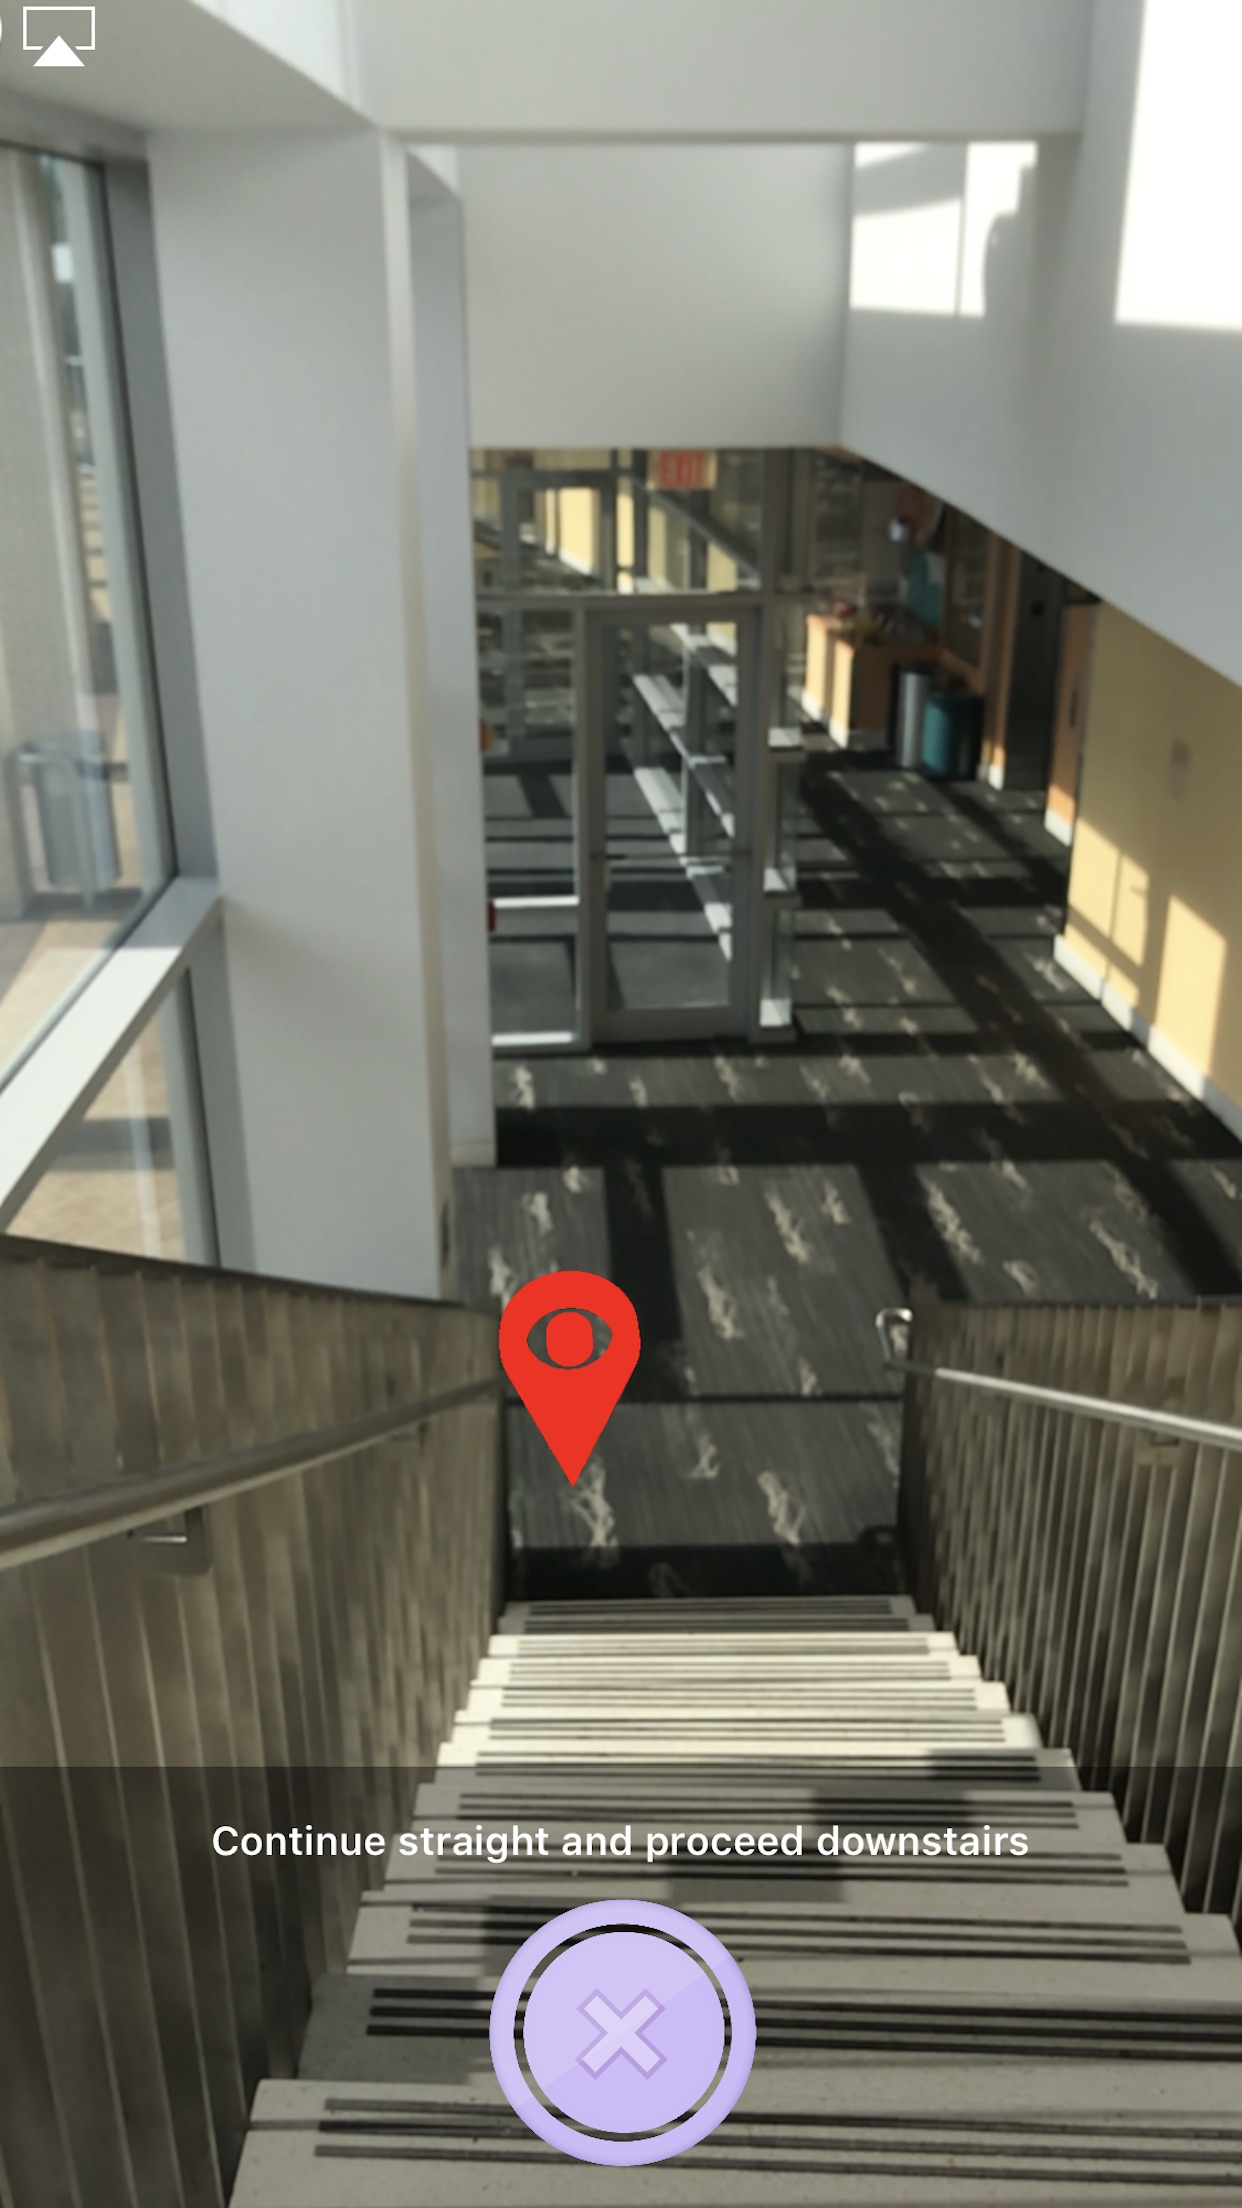
\includegraphics[width=0.48\linewidth]{Figures/clew_screenshot_1}\hspace{.03\linewidth}
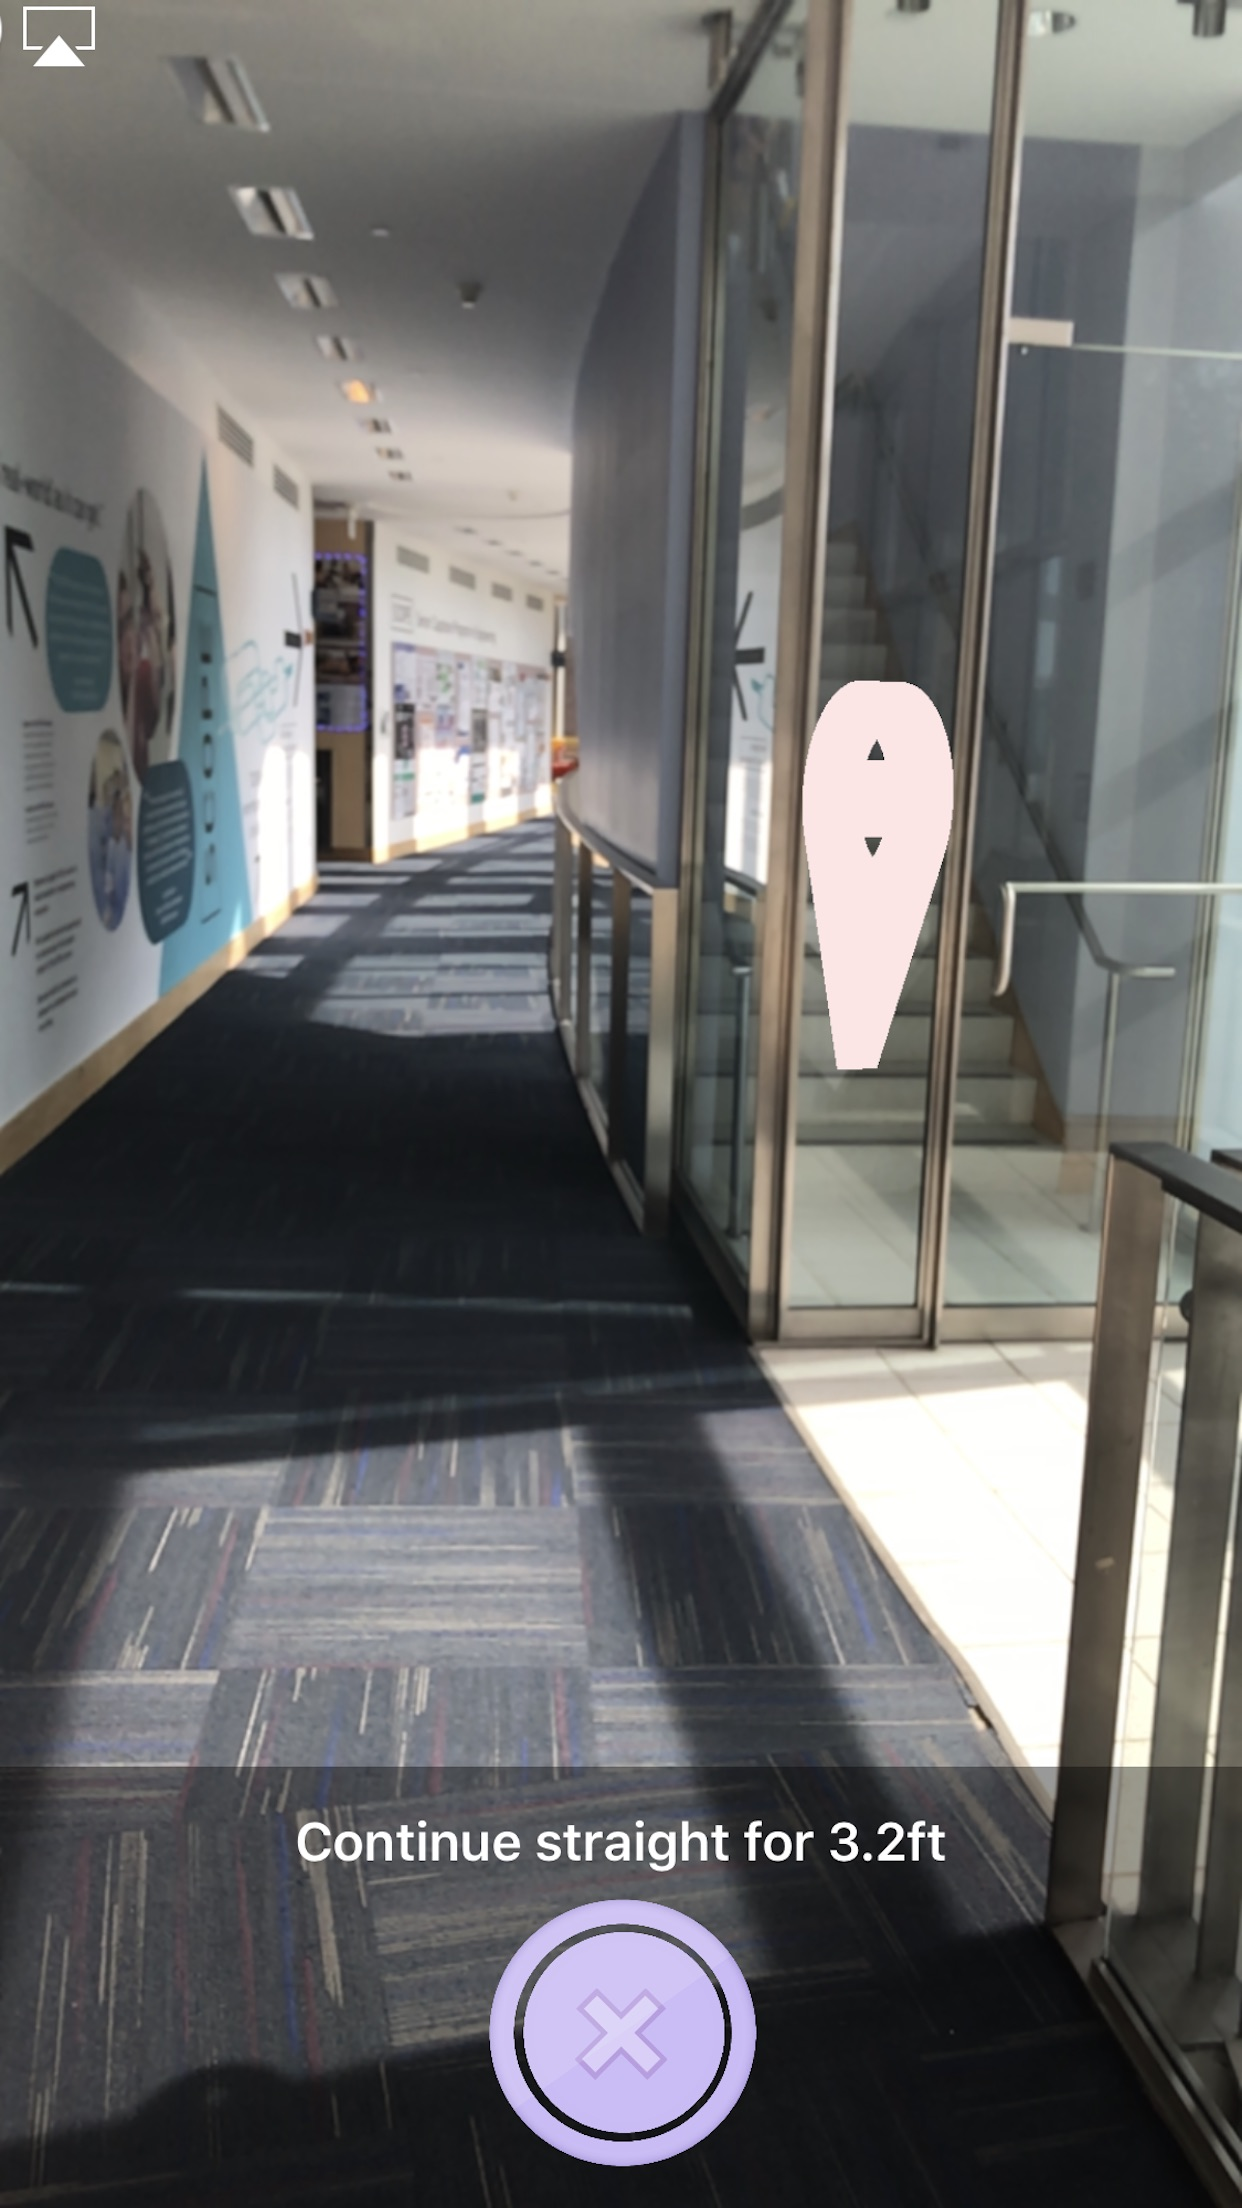
\includegraphics[width=0.48\linewidth]{Figures/clew_screenshot_2}
\end{center}
\caption{Two screenshots from our app ``Clew.'' Both images show the app in navigation mode where a user is using the app to retrace a route they have previously traveled.  The text for the left image says ``Continue straight and proceed downstairs'' and the text on the right says ``Continue straight for 3.2 feet.''\label{fig:clewshots}}
\end{figure}

\begin{enumerate}
\item Basic idea of the app
\item Co-design elements
\item Lack of suitability for guide dog travel
\item Path recording (including Douglas-Ramer-Peucker algorithm \cite{douglas1973algorithms} (cool page for generating examples of the algorithm running http://karthaus.nl/rdp/))
\item Path following (including feedback mechanisms)
\item Pause feature
\item Usability test
\end{enumerate}

\section{ViewShare: an app for Object Finding in Challenging Environments}
Todo: connect to idea of sense of space and building mental maps.
\begin{enumerate}
\item Basic idea  of the app
\item Co-design elements
\item Overview of the 3D location mechanism
\item App for the searcher
\begin{enumerate}
\item Speech interface
\item Automatic snapshotting
\item Guidance to object (3D versus 2D feedback)
\end{enumerate}
\item App for the finder
\begin{enumerate}
\item Description of general interface
\item Special interface for triangulation
\end{enumerate}
\item Usability test
\end{enumerate}

\section{Discussion and Future Work}
\begin{enumerate}
\item Interpretation of the results
\item Future work for each of the apps
\begin{enumerate}
\item New feature development
\item Robust usability testing
\end{enumerate}
\item Unresolved Issues
\item Promises of AR technology
\item Limitations of AR technology
\begin{enumerate}
\item Accuracy
\item Accessibility to voice over (minor problem, but worth mentioning)
\end{enumerate}
\end{enumerate}

\section{Conclusion}
We have presented two smartphone apps that each allow people who are B/VI to perform significant, new tasks with their smartphones.  In contrast to the typical use cases of indoor navigation and image process where smartphones have provided significant value for users who are B/VI, our apps provide some of the first apps that can be used for navigation and object finding in arbitrary indoor environments.  While the initial results of our usability test are promising, much more work is required to refine the developed apps to be maximally useful to the B/VI community.

Further, we have outlined several promising areas of opportunity for the development of new augmented reality-enabled apps to support people who are B/VI.  We have also provided a discussion of the limitations of this technology.  With a combination of the development of new algorithms, careful co-design with users who are B/VI, and the improvement of the underlying AR capabilities from smartphone vendors these limitations can hopefully be overcome to create impactful new assistive smartphone technology for people who are B/VI.  

\section{Acknowledgments}
Removed for anonymous review.

% BALANCE COLUMNS
\balance{}

\newpage
% REFERENCES FORMAT
% References must be the same font size as other body text.
\bibliographystyle{SIGCHI-Reference-Format}
\bibliography{../references/assets,../references/assistive_tech,../references/disability_studies,../references/machine_learning}

\end{document}

%%% Local Variables:
%%% mode: latex
%%% TeX-master: t
%%% End:
